\chapter{Modelling Class Densities in a Frozen Feature Space}
\label{methodology}

\section{Proposed Architecture}

As shown in Figure~\ref{fig:architecture}, our CIL framework is built upon a simple yet structurally motivated decomposition: (i) a frozen feature extractor based on a visual foundation model, and (ii) a probabilistic classification layer that models each object category through an independent Gaussian distribution in the embedding space. Given an input image, the feature extractor maps it to a fixed high-dimensional representation. For each class, we maintain a class-conditional multivariate Gaussian characterized by its mean vector and covariance matrix, estimated incrementally from observed samples. Classification is performed according to the maximum likelihood principle, assigning the input to the class whose Gaussian model yields the highest likelihood under the stationary embedding representation. This modular separation between representation learning and statistical modeling enables incremental updates without backpropagation or parameter adaptation: adding a new class requires only estimating its distribution in the fixed feature space, while previously learned classes remain unaffected at the representation level.

\begin{figure}[htb]
	\centering
	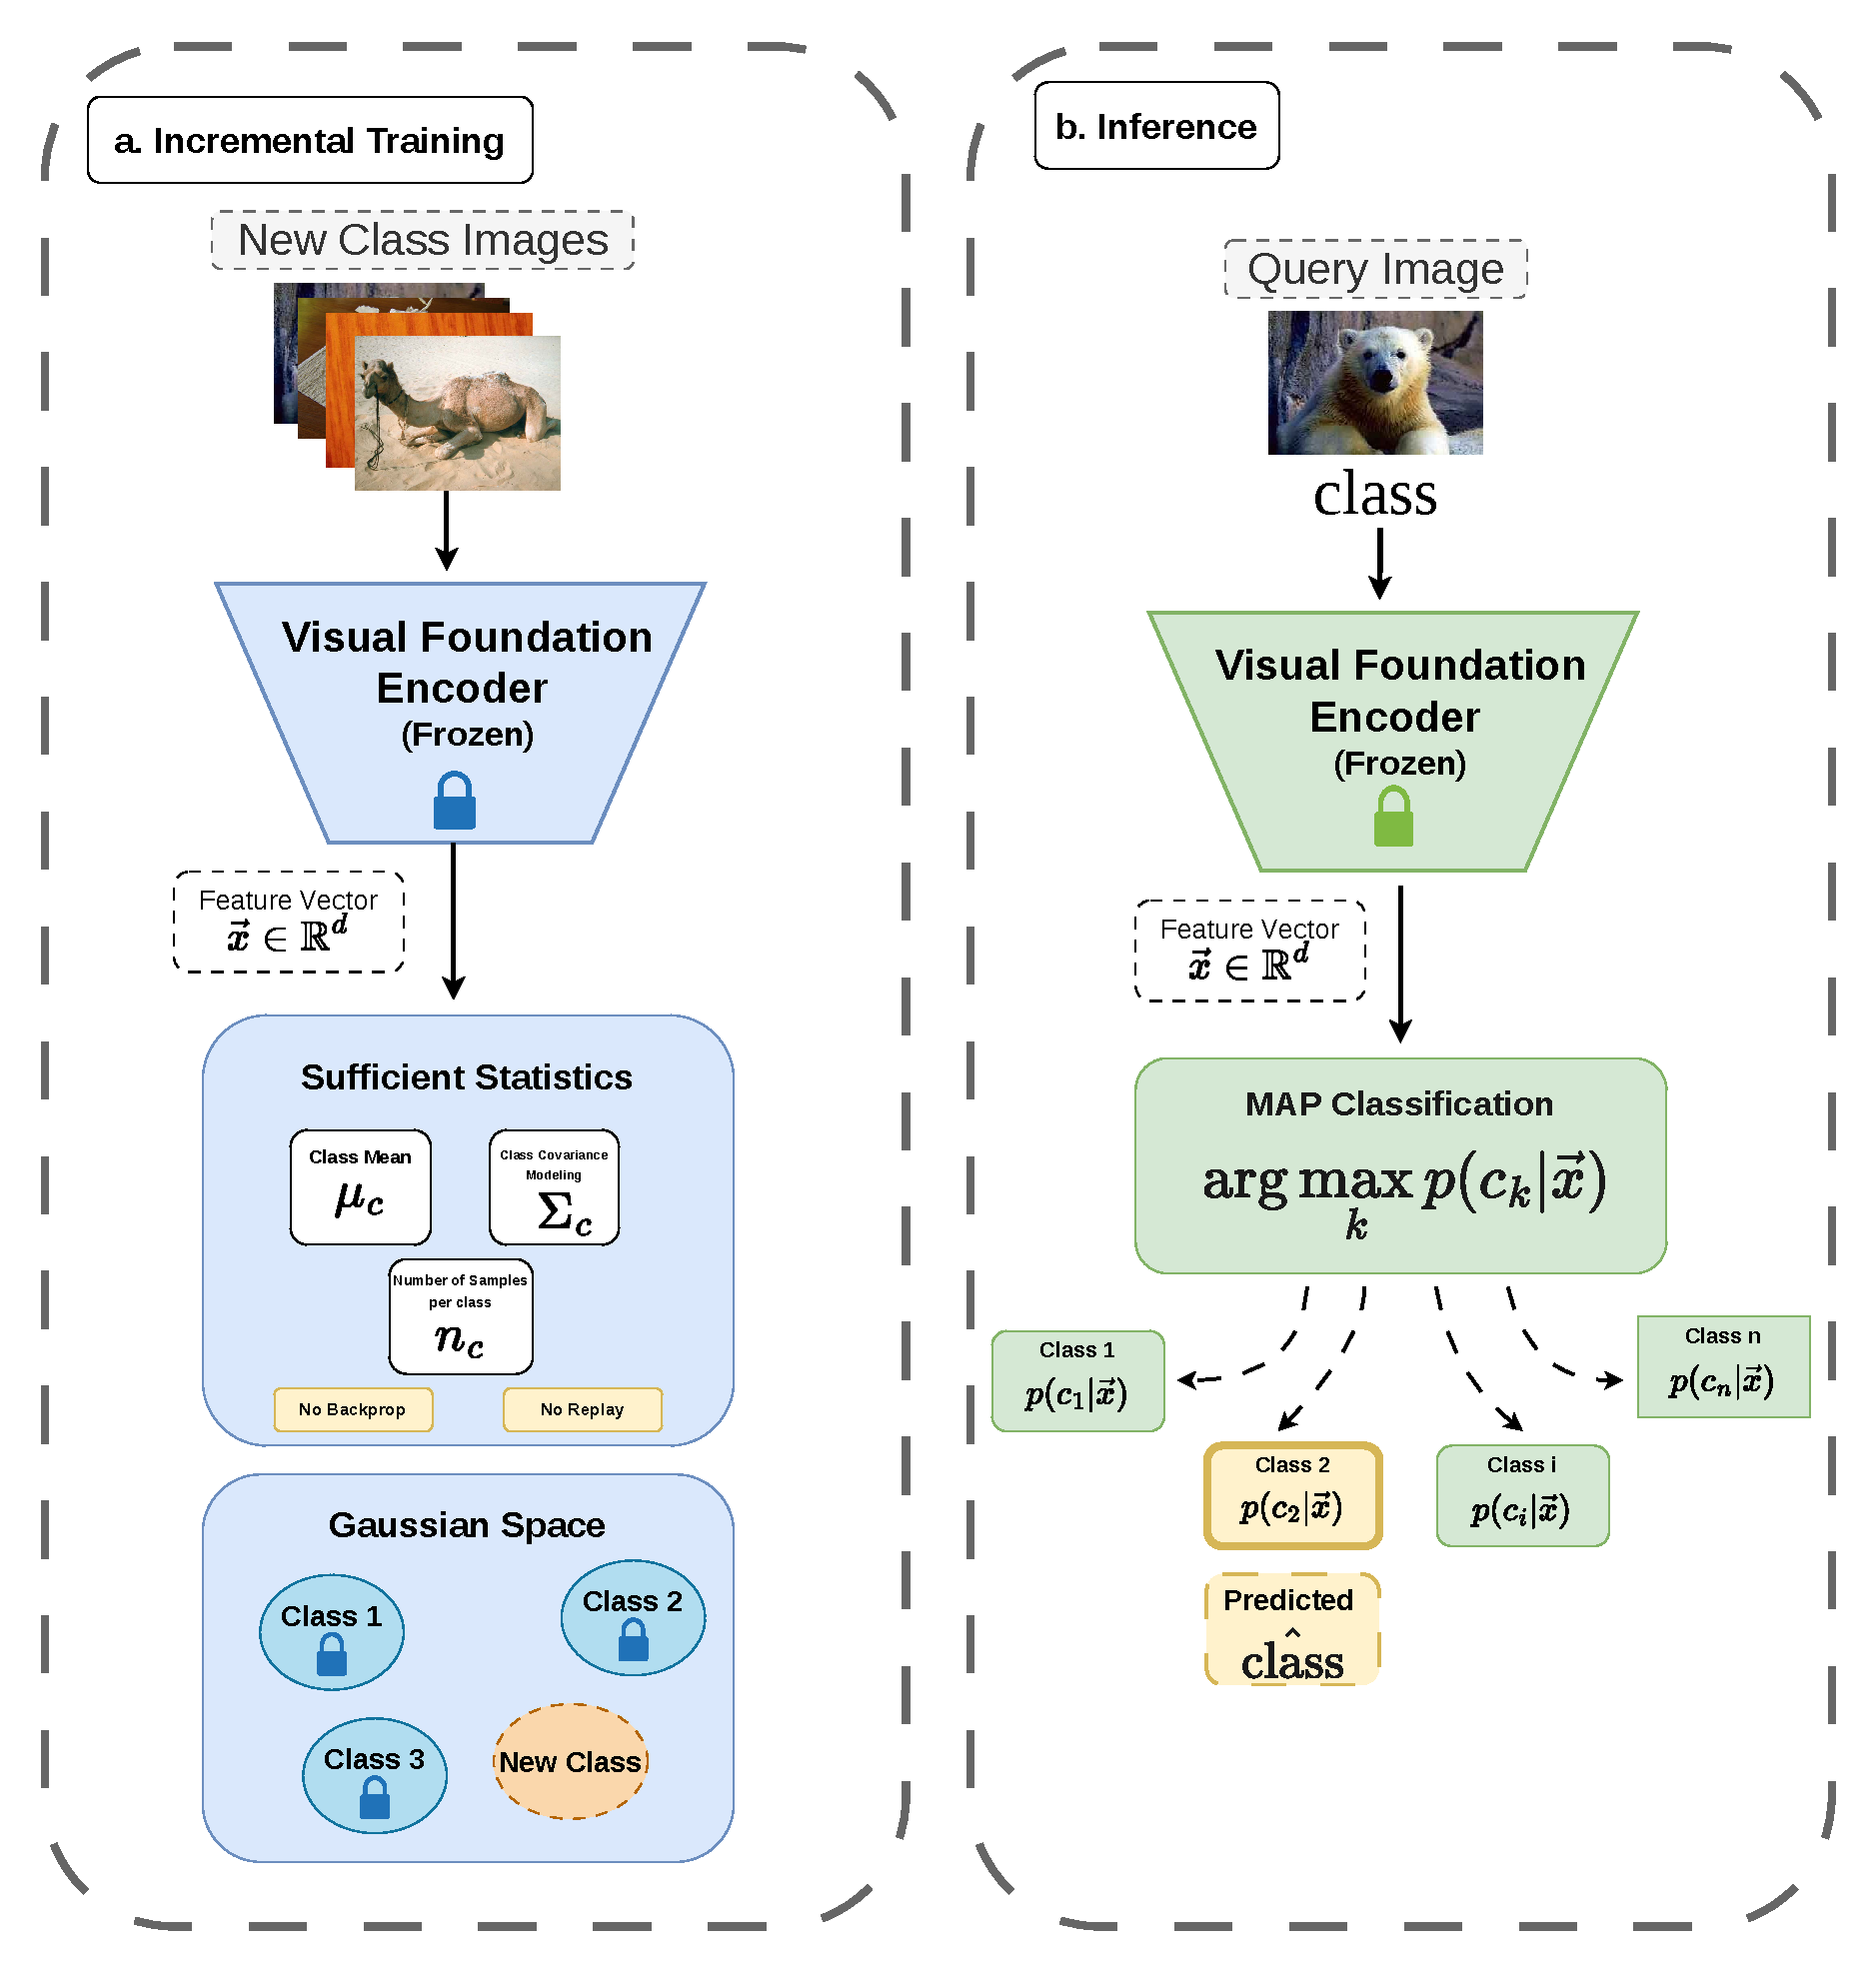
\includegraphics[width=0.6\textwidth]{imagenes/methodology/TMLR_block_diagram_approach.pdf}
	\caption{Overview of the proposed framework, reproduced from the peer-reviewed article that accompanies this thesis. A frozen foundation encoder maps each input image to a fixed embedding $\vec{x}\in\mathbb{R}^d$. Each class is represented by a Gaussian density (mean and covariance) that is updated incrementally without backpropagation. At inference, classification follows the MAP rule under the learned class-conditional densities. This diagram supersedes the general conceptual schematic used purely for narrative context in the Introduction (Figure~\ref{fig:intro_overview}), adding explicit detail on the recursive statistic-update mechanism shared by all covariance parameterisations introduced in Section~\ref{sec:covariance_estimation}.}
	\label{fig:architecture}
\end{figure}

\subsection{Likelihood-Based Classification}
\label{sec:method:classification}

Given an input image $x \in \mathcal{X}$, the frozen foundation model $\mathcal{F}$ produces a fixed-dimensional embedding
\begin{equation}
    \vec{x} = \mathcal{F}(x) \in \mathbb{R}^d
    \label{eq:feature_extractor}
\end{equation}
and all learning is performed directly in the stationary feature space $\mathbb{R}^d$. We adopt a generative modelling framework and assume class-conditional Gaussian feature distributions:
\begin{equation}
    p(\vec{x} \mid y = c) = \mathcal{N}(\vec{x} \mid \boldsymbol{\mu}_c,\, \boldsymbol{\Sigma}_c),
    \label{eq:class_gaussian}
\end{equation}
where $\boldsymbol{\mu}_c \in \mathbb{R}^d$ and $\boldsymbol{\Sigma}_c \succ 0$ are the class-specific mean and covariance matrix, estimated incrementally from observed samples. Classification is performed via Maximum A Posteriori (MAP) inference:
\begin{equation}
    \hat{y} = \arg\max_{c \in \mathcal{Y}} \left[ \log p(\vec{x} \mid y=c) + \log \pi_c \right],
    \label{eq:map}
\end{equation}
where $\pi_c = p(y=c)$ is the class prior. Under a uniform prior and the Gaussian density model, the decision rule is equivalent to the quadratic discriminant:
\begin{equation}
    \hat{y} = \arg\min_{c \in \mathcal{Y}} \left[ (\vec{x} - \boldsymbol{\mu}_c)^T \boldsymbol{\Sigma}_c^{-1} (\vec{x} - \boldsymbol{\mu}_c) + \log|\boldsymbol{\Sigma}_c| \right].
    \label{eq:qda}
\end{equation}
This quadratic decision function is the core of the proposed framework. The Mahalanobis term $(\vec{x}-\boldsymbol{\mu}_c)^T\boldsymbol{\Sigma}_c^{-1}(\vec{x}-\boldsymbol{\mu}_c)$ encodes the \emph{shape} of the class distribution while $\log|\boldsymbol{\Sigma}_c|$ encodes its \emph{volume}. The covariance parameterisations introduced in Section~\ref{sec:covariance_estimation} are specialisations of Equation~\eqref{eq:qda} that differ in the structure imposed on $\boldsymbol{\Sigma}_c$; the interplay between the shape and volume components is the central design axis of the covariance estimation study and is examined in detail in the analysis of results.

Adding a new class to the system requires only estimating the sufficient statistics $(\boldsymbol{\mu}_c, \boldsymbol{\Sigma}_c)$ in the fixed feature space; previously learned class statistics are never modified. This formulation therefore enables genuinely incremental updates without backpropagation, replay buffers, or exemplar storage.

\subsection{Datasets and Experimental Protocol}
We follow the standard Continual Learning (CL) protocol where the model learns a sequence of disjoint tasks and calculates the average accuracy and the forgetting. The specific configurations for the datasets are as follows:

\begin{itemize}
	\item \textbf{Split CIFAR-100:} This dataset is a widely utilized benchmark in the continual learning literature. It partitions the original CIFAR-100 \cite{cifar100} dataset into 10 disjoint tasks, with each task containing 10 distinct classes.

	\item \textbf{Split ImageNet-R:} This benchmark is constructed from ImageNet-R \cite{imagenetR}, a dataset containing renditions of ImageNet classes such as art, cartoons, and sketches. We randomly divide the 200 classes into 10 sequential tasks, with 20 classes per task, introducing a significant domain shift challenge.

	\item \textbf{Split Caltech-256:} Designed to evaluate the model on higher-resolution images with greater object variability, this benchmark utilises the Caltech-256 \cite{caltech256} dataset. The first 250 of the original 256 categories are used and sequentially divided into 10 disjoint tasks of 25 classes each; the remaining six categories are discarded so that the benchmark has a fixed, balanced number of classes per task. The resulting protocol contains approximately 28\,100 images with an average of $\overline{n_c}\!\approx\!112$ training samples per class, which makes the per-class budget the smallest of the three constituent datasets and stresses the high-dimensional covariance estimators introduced in Section~\ref{sec:covariance_estimation}.

	\item \textbf{Split Joint Dataset:} This benchmark serves as a comprehensive stress test by aggregating the 30 tasks from the three aforementioned datasets into a single, heterogeneous stream. The tasks are presented to the system in a randomized order, forcing the model to navigate extreme distribution shifts between natural, artistic, and high-resolution images. This long-horizon sequence is specifically designed to evaluate the model's resilience against catastrophic forgetting over an extended period of diverse learning objectives.
\end{itemize}

\subsection{Model Metrics}

As mentioned, to quantify performance, SOTA works \cite{wang2022learning} utilize two standard metrics derived from the test accuracy scores: the average accuracy and the average forgetting.

On the one hand, \textbf{Average Accuracy ($A_t$)}, presented on equation \eqref{eq_AA}, measures overall performance after task $t$. It is the mean test accuracy across all tasks learned up to that point.

\begin{equation}
	A_t = \frac{1}{t} \sum_{\tau=1}^{t} S_{t,\tau}
	\label{eq_AA}
\end{equation}

On the other hand, \textbf{Forgetting ($F_{t}$)}, presented on equation \eqref{eq_AF}, quantifies how much the model has forgotten earlier tasks. It computes, for each past task, how much accuracy has dropped compared to its best historical score, and averages those drops.

\begin{equation}
	F_t = \frac{1}{t-1} \sum_{\tau=1}^{t-1} \left( \max_{k \le t-1} S_{k,\tau} - S_{t,\tau} \right)
	\label{eq_AF}
\end{equation}

Regarding forgetting, the proposed framework does not exhibit forgetting in the conventional sense, as previously learned class statistics are never modified when new classes are introduced. The measured forgetting values therefore primarily reflect the increased classification difficulty as the number of competing classes grows, rather than degradation of previously learned representations.

With the architecture, benchmarks and evaluation metrics now in place, the remainder of this chapter follows a single, consistent narrative arc that Chapter~\ref{ch:results} mirrors section by section: it opens with the covariance-estimation methodology and its mixture-of-Gaussians extensions, then introduces the probabilistic confidence and calibration metrics that complement raw accuracy, followed by the incremental class-inclusion protocol that stresses the growing decision surface. It then turns to the inter-class pairwise Bhattacharyya distance, which quantifies the separability of the learned class-conditional Gaussians, before examining the sensitivity of the framework to the choice of upstream backbone and the spectral structure of the embedding space it produces. The chapter closes with the statistical validation of the Gaussianity assumption on which the whole framework rests.

\section{Covariance Estimation}
\label{sec:covariance_estimation}

Due to the high dimensionality of the extracted feature ($\vec{x}\in \mathbb{R}^d$), the empirical sample covariance matrix (SCM) is a poor estimator for each class: its eigenvalues are biased, and the matrix is singular whenever $n_c < d$. In our setting $d = 768$ while $n_c$ ranges from approximately $40$ to $400$ depending on the benchmark, so the matrix always has at most $n_c - 1$ non-zero eigenvalues out of $d = 768$, leaving $d - (n_c - 1)$ eigenvalues that are structurally zero before any regularisation is applied.
The Gaussian modelling assumption that motivates the covariance-based classifiers introduced below is formally validated later in Section~\ref{sec:method:gaussianity_main}; here we focus on how to obtain a well-conditioned covariance estimate under that assumption. Our benchmarks are tested using different covariance estimation methods:

\subsection{Diagonal Covariances}
In this configuration, we assume that the features within each class $c$ are independent, leading to a diagonal covariance matrix $\boldsymbol{\Sigma}_c = \text{diag}(\sigma_{c,1}^2, \sigma_{c,2}^2, \dots, \sigma_{c,d}^2)$. This simplification significantly reduces the number of parameters to estimate from $O(d^2)$ to $O(d)$, which is particularly advantageous when the dimensionality $d = 768$ is large relative to the number of samples per class. For each class $c \in \{1, \dots, C\}$, the mean vector $\boldsymbol{\mu}_c$ and the diagonal elements of $\boldsymbol{\Sigma}_c$ are computed as:

\begin{equation}
	\boldsymbol{\mu}_c = \frac{1}{n_c} \sum_{i=1}^{n_c} \vec{x}_i, \quad \sigma_{c,j}^2 = \frac{1}{n_c-1} \sum_{i=1}^{n_c} (x_{i,j} - \mu_{c,j})^2 + \epsilon
\end{equation}
where $\epsilon = 10^{-6}$ is a small constant added to ensure numerical stability and strictly positive variances. The log-likelihood of a test sample $\vec{x}$ belonging to class $c$ is determined by the discriminant function:

\begin{equation}
	g_c(\vec{x}) = \ln P(\vec{x}|c) + \ln P(c)
\end{equation}

Under the assumption of a uniform prior $P(c)$ and Gaussian distribution, this simplifies to:

\begin{equation}
	g_c(\vec{x}) = -\frac{1}{2} \sum_{j=1}^{d} \left( \ln(2\pi\sigma_{c,j}^2) + \frac{(x_j - \mu_{c,j})^2}{\sigma_{c,j}^2} \right)
\end{equation}


\subsection{Full Covariances}
\label{sec:method:full_cov}

To account for the dependencies between different dimensions of the feature vector, we estimate a full covariance matrix $\boldsymbol{\Sigma}_c \in \mathbb{R}^{d \times d}$ for each class $c$. While this provides a richer representation of the class distribution, the estimation of $d^2$ parameters is prone to ill-conditioning when the number of samples $n_c$ is limited.The mean vector $\boldsymbol{\mu}_c$ and the empirical covariance $\boldsymbol{\Sigma}_c$ are calculated as:

\begin{equation}
	\boldsymbol{\mu}_c = \frac{1}{n_c} \sum_{i=1}^{n_c} \vec{x}_i, \quad \boldsymbol{\Sigma}_c = \frac{1}{n_c - 1} \sum_{i=1}^{n_c} (\vec{x}_i - \boldsymbol{\mu}_c)(\vec{x}_i - \boldsymbol{\mu}_c)^T
\end{equation}

To ensure that the matrix is invertible and to improve numerical stability, a regularization is applied by adding a small identity term to the diagonal: $\hat{\boldsymbol{\Sigma}}_c = \boldsymbol{\Sigma}_c + \epsilon I$, with $\epsilon = 10^{-6}$.

For obtaining the precision matrix $Q_c$ (the inverse of the covariance matrix $\hat{\boldsymbol{\Sigma}}_c$), an approach based on Cholesky decompositions is used. The covariance $\hat{\boldsymbol{\Sigma}}_c$ is decomposed as
\begin{equation}
	\hat{\boldsymbol{\Sigma}}_c = C_c C_c^T, \qquad C_c L_c = I,
	\label{eq:cholesky_decomp}
\end{equation}
with $C_c$ lower triangular and $I$ the identity, so that $L_c = C_c^{-1}$ is the Cholesky factor of the precision matrix $Q_c = L_c^T L_c$.

Then, the squared Mahalanobis distance and the log-determinant are computed from $\boldsymbol{\mu}_c$ and $L_c$ as:

\begin{equation}
	d_M(\vec{x}, \boldsymbol{\mu}_c, L_c) = (\vec{x} L_c - \boldsymbol{\mu}_c L_c)^T (\vec{x} L_c - \boldsymbol{\mu}_c L_c)
	\label{eq:cholesky_mahalanobis}
\end{equation}

\begin{equation}
	\ln |\hat{\boldsymbol{\Sigma}}_c| = 2 \sum_{i=1}^{d}{\ln(L_{c \, i,i})}
	\label{eq:cholesky_logdet}
\end{equation}

\subsection{Hybrid Covariance}
\label{sec:method:hybrid_cov}

The hybrid covariance estimator decouples the squared Mahalanobis distance from its associated normalisation constant. For each class $c$, the full covariance matrix $\hat{\boldsymbol{\Sigma}}_c$ is estimated and regularised exactly as in Section~\ref{sec:method:full_cov}, and the squared Mahalanobis distance $d_M(\vec{x}, \mu_c, L_c)$ is computed using the same Cholesky-based procedure of Equations~\eqref{eq:cholesky_decomp}--\eqref{eq:cholesky_mahalanobis}, so that the \emph{shape} of the discriminant retains the full off-diagonal structure of the empirical covariance. However, the log-determinant term---which represents the \emph{volume} of the distribution---is computed using only the diagonal elements (variances) of the covariance matrix:
\begin{equation}
	\ln |\hat{\boldsymbol{\Sigma}}_c|_{\text{diag}} = \sum_{j=1}^{d} \ln(\sigma_{c,j}^2),
	\label{eq:hybrid_logdet}
\end{equation}
where $\sigma_{c,j}^2$ denotes the $j$-th diagonal entry of $\hat{\boldsymbol{\Sigma}}_c$. The resulting discriminant function is defined as:
\begin{equation}
	g_c(\vec{x}) = -\frac{1}{2} \left( d \ln(2\pi) + \sum_{j=1}^{d} \ln(\sigma_{c,j}^2) + d_M(\vec{x}, \boldsymbol{\mu}_c, L_c) \right).
	\label{eq:hybrid_discriminant}
\end{equation}

This formulation avoids the numerical issues that arise when near-zero eigenvalues of $\hat{\boldsymbol{\Sigma}}_c$ artificially inflate or destabilise the exact log-determinant, at the cost of using a diagonal approximation for the volume term only.

\subsection{OAS Covariance}
\label{sec:method:oas}

Oracle Approximating Shrinkage (OAS) is a shrinkage technique that computes an structurally optimized covariance matrix by finding an optimal compromise between the sample covariance matrix and a structured target (the identity matrix scaled by the average trace).The OAS estimator provides a more accurate estimation of the covariance $\boldsymbol{\Sigma}_c$ by minimizing the Mean Squared Error (MSE) under the assumption of Gaussianity. The estimated covariance is defined as:

\begin{equation}
	\hat{\boldsymbol{\Sigma}}_{\text{OAS}, c} = (1 - \rho_c) \hat{\boldsymbol{\Sigma}}_{\text{SCM}, c} + \rho_c \hat{F}_c
\end{equation}
where $\rho_c$ is the shrinkage coefficient calculated specifically for class $c$, $\hat{\boldsymbol{\Sigma}}_{\text{SCM}, c}$ is the sample covariance matrix, and $\hat{F}_c = \frac{\text{tr}(\hat{\boldsymbol{\Sigma}}_{\text{SCM}, c})}{d} I$ is the shrinkage target.In our implementation, we compute the precision matrix $\Psi_c = \hat{\boldsymbol{\Sigma}}_{\text{OAS}, c}^{-1}$ directly via the OAS algorithm. This precision matrix is then used to calculate the Mahalanobis distance in the log-likelihood discriminant function:

\begin{equation}
	g_c(\vec{x}) = \ln A_c - \frac{1}{2} (\vec{x} - \boldsymbol{\mu}_c)^T \Psi_c (\vec{x} - \boldsymbol{\mu}_c)
\end{equation}

where $\ln A_c$ is the normalization constant derived from the log-determinant of the OAS-estimated covariance matrix, evaluated numerically via the stable log-determinant of the eigendecomposition. This approach ensures that the model captures class-specific correlations while remaining robust to the ``curse of dimensionality.''

\subsection{Ledoit-Wolff}
\label{sec:method:ledoitwolf}

The Ledoit-Wolf Diagonal Anchor estimator addresses the instability of the sample covariance matrix $S$ by shrinking it toward a target matrix $T$.

The selection of a target matrix $T$ represents a prior assumption regarding the feature distribution. Both methods stabilize the estimator by pulling the noisy off-diagonal elements of the sample covariance matrix $S$ toward zero, but they differ in how they treat the diagonal elements (the variances).

\subsubsection{Diagonal Target}
The diagonal anchor is defined as $T_{\text{diag}} = \text{diag}(s_{11}, s_{22}, \dots, s_{dd})$. This approach assumes that the features are independent but allows for heteroscedasticity, meaning each dimension can have a different variance. Shrinkage toward this target preserves the scale of each individual feature as observed in the sample data while suppressing only the correlations. This is particularly useful when certain dimensions of the DINOv2 embeddings are naturally more informative or volatile than others.

\subsubsection{Identity Target}The identity anchor is more restrictive, defined as $T_{\text{ident}} = \mu I$, where $\mu = \frac{1}{d} \text{tr}(S)$ is the average variance across all dimensions. This target assumes that the features are not only independent but also share a common variance (homoscedasticity). The resulting distribution is spherical. Because the embeddings used in this work are L2-normalized, the variances across dimensions tend to be similar, making the identity anchor a highly robust regularizer that prevents any single dimension from disproportionately influencing the distance metric.

\subsubsection{Structural Summary}The fundamental difference between these two estimators lies in the flexibility of the variance components:

\begin{itemize}
	\item \textbf{Diagonal Anchor:} $\hat{\Sigma}_{ij} = (1-\gamma)s_{ij}$ for $i \neq j$, and $\hat{\Sigma}_{ii} = s_{ii}$. It yields an axis-aligned ellipsoidal distribution.
	\item \textbf{Identity Anchor:} $\hat{\Sigma}_{ij} = (1-\gamma)s_{ij}$ for $i \neq j$, and $\hat{\Sigma}_{ii} = (1-\gamma)s_{ii} + \gamma \mu$. It yields a distribution that is pulled toward a perfectly spherical geometry.
\end{itemize}

\subsection{Shared Covariance}
\label{subsec:shared_cov_original}

The Shared Covariance framework assumes that the internal noise or feature variability is homoscedastic across all classes. In this paradigm, all classes share a single covariance matrix $\boldsymbol{\Sigma}$, which captures the global structure of the feature space.

A key aspect of this framework in the continual learning setting is that $\boldsymbol{\Sigma}$ is re-estimated at the end of each task $t$ using only the classes observed so far, $\mathcal{C}_t = \{1, \dots, C_t\}$.

\section{Mixture of Gaussians}

In order to capture potential multi-modality within the feature space of a single class, we employ Gaussian Mixture Models (GMM). We implemented the following models using the previously defined diagonal, full and hybrid covariances approaches.

\subsection{Mixture of 2 Gaussians}

Forcing each class to be defined as a GMM with $K=2$ components, each class $c$ can be modeled by a probability density function:

\begin{equation}
	p(\vec{x}|c) = \sum_{k=1}^{K} \pi_{c,k} \mathcal{N}(\vec{x} | \boldsymbol{\mu}_{c,k}, \boldsymbol{\Sigma}_{c,k})
\end{equation}

where $\pi_{c,k}$ represents the mixing weight of the $k$-th component for class $c$, subject to $\sum \pi_{c,k} = 1$. In this specific variant, the covariance matrices $\boldsymbol{\Sigma}_{c,k}$ are restricted to be diagonal to maintain computational efficiency and prevent over-fitting in the high-dimensional DINOv2 space.The parameters $\{\pi_{c,k}, \boldsymbol{\mu}_{c,k}, \boldsymbol{\Sigma}_{c,k}\}$ are estimated using the Expectation-Maximization (EM) algorithm. To ensure numerical stability, a small constant $\epsilon = 10^{-5}$ is added to the diagonal of each covariance matrix. The log-likelihood for a test sample $\vec{x}$ is calculated using the \textit{LogSumExp} operator to avoid underflow:

\begin{equation}
	\ln p(\vec{x}|c) = \text{lnaddexp} \left( \ln(\pi_{c,1} \mathcal{N}(\vec{x} | \boldsymbol{\mu}_{c,1}, \boldsymbol{\Sigma}_{c,1})), \ln(\pi_{c,2} \mathcal{N}(\vec{x} | \boldsymbol{\mu}_{c,2}, \boldsymbol{\Sigma}_{c,2})) \right)
\end{equation}

In the implementation, this is expanded as:

\begin{equation}
	\ln p(\vec{x}|c) = \ln \left( \exp( \ln \pi_{c,1} + \ln A_{c,1} - \frac{1}{2} d_{M,1} ) + \exp( \ln \pi_{c,2} + \ln A_{c,2} - \frac{1}{2} d_{M,2} ) \right)
\end{equation}

where $d_{M,k}$ is the diagonal Mahalanobis distance to the $k$-th component and $\ln A_{c,k}$ is the normalization constant. This approach allows the model to better represent classes that may contain significantly different visual sub-types or clusters within the latent embedding space.


\subsection{Mixture of up-to-4 Gaussians}

To adapt to the varying complexity of different classes within the different datasets, we implement a flexible Gaussian Mixture Model where the number of components $K_c$ for each class $c$ is not fixed. Instead, the model selects the most appropriate number of components $K_c \in \{1, 2, 3, 4\}$ by minimizing the Bayesian Information Criterion (BIC).The BIC is defined as:

\begin{equation}
	\text{BIC} = \ln(n)k - 2\ln(\hat{L})
	\label{eq:bic_mog4}
\end{equation}

where $n$ is the number of samples in the class, $k$ is the number of free parameters to be estimated, and $\hat{L}$ is the maximized value of the likelihood function. By using diagonal covariance matrices, the number of parameters per component is kept low ($2d + 1$), allowing the selection process to favor multi-modal distributions only when the increase in likelihood justifies the additional parameters. For each component $k$ in class $c$, the diagonal covariance $\boldsymbol{\Sigma}_{c,k} = \text{diag}(\sigma_{c,k,1}^2, \dots, \sigma_{c,k,d}^2)$ is regularized with $\epsilon = 10^{-6}$. The classification of a test sample $\vec{x}$ involves calculating the weighted log-likelihood across all active classes:

\begin{equation}
	\ln p(\vec{x}|c) = \text{LSE}_{k=1}^{K_c} \left( \ln \pi_{c,k} - \frac{1}{2} \left( \sum_{j=1}^{d} \ln(2\pi\sigma_{c,k,j}^2) + \sum_{j=1}^{d} \frac{(x_j - \mu_{c,k,j})^2}{\sigma_{c,k,j}^2} \right) \right)
\end{equation}

where $\text{LSE}$ denotes the LogSumExp operator. This methodology allows for a more granular representation of class distributions—using a single Gaussian for simple, compact classes and up to four Gaussians for classes with high intra-class variance or distinct visual sub-clusters—while preserving the numerical efficiency of diagonal estimators.

\section{Confidence and Calibration Metrics}
\phantomsection\label{sec:method:metrics}

While accuracy and forgetting measure the correctness of predictions, they do not account for the model's reliability or its tendency to over-confide in incorrect decisions---a common issue in Class-Incremental Learning. To address this, we introduce five complementary metrics that jointly characterise the probabilistic behaviour of the classifier: the Expected Calibration Error (ECE) measures the global alignment between confidence and accuracy; the Confidence on Errors (CoE) quantifies how dangerously overconfident the model is when it fails; Total Confidence (TC) and Probability Margin (PM) both capture the decisiveness of the posterior distribution from two complementary angles; and the Average Predictive Entropy ($H$) measures the spread of probability mass across all classes.

\subsection{Expected Calibration Error (ECE)}
This metric quantifies the mismatch between predictive confidence and empirical accuracy. We partition the predictions into $M$ equally spaced bins based on their confidence scores. The ECE is defined as the weighted average of the absolute difference between the accuracy and confidence of each bin:

\begin{equation}
	ECE_t = \sum_{m=1}^{M} \frac{|B_m|}{N} \left| acc(B_m) - conf(B_m) \right|\label{eq_ECE}
\end{equation}

where $N$ is the total number of samples, $B_m$ is the set of indices of samples whose prediction confidence falls into the $m$-th interval, and $acc(B_m)$ and $conf(B_m)$ represent the mean accuracy and mean confidence within that bin, respectively.

\subsection{Confidence on Errors (CoE)}
To specifically analyze the model's behavior when it fails, we measure the average confidence assigned to the winning (but incorrect) class. High CoE indicates a model that is ``dangerously wrong'', which is a critical factor in safety-oriented applications. It is computed for a task $t$ as:

\begin{equation}
	CoE_t = \frac{1}{|\mathcal{E}_t|} \sum_{i \in \mathcal{E}_t} \max(\hat{p}_i)
\end{equation}

where $\mathcal{E}_t$ is the set of misclassified samples and $\hat{p}_i$ is the predicted probability distribution for sample $i$.

\subsection{Total Confidence (TC)}

Total Confidence measures how certain the model is on average about its top-1 prediction, regardless of whether that prediction is correct:

\begin{equation}
	TC_t = \frac{1}{N} \sum_{i=1}^{N} \max_{c} \, p_{i,c}
\end{equation}

A value of $TC=1$ means the model assigns all probability mass to a single class for every sample---it is always maximally decisive. A value close to $1/C$ would indicate near-uniform posteriors. TC is a measure of \emph{decisiveness}, not correctness: a well-calibrated model should have $TC \approx A_T$ (confident when right, uncertain when wrong), whereas a pathologically overconfident model can reach $TC \approx 1$ even at low accuracy.

\subsection{Probability Margin (PM)}

The Probability Margin is the natural, non-logarithmic measure of how decisively the model separates its top-1 prediction from its second-best alternative:

\begin{equation}
	PM_t = \frac{1}{N} \sum_{i=1}^{N} \Bigl( p_{i,(1)} - p_{i,(2)} \Bigr)
\end{equation}

where $p_{i,(1)} \ge p_{i,(2)}$ are the two highest posterior probabilities for sample $i$. A margin near $1$ means the model almost entirely ignores its second candidate; a margin near $0$ means the model is nearly tied between its top-two guesses and one should treat the prediction with caution. PM is bounded in $[0,1]$ and directly interpretable: a value of $0.7$ means the winning class is, on average, assigned $70\%$ more probability than the runner-up.

\subsection{Average Predictive Entropy ($H$)}
We utilize Shannon entropy to measure the uncertainty of the model's predictions. A higher entropy suggests that the model is distributing its probability mass across multiple classes, indicating lower certainty. For task $t$, the average entropy is calculated as:

\begin{equation}
	H_t = \frac{1}{N} \sum_{i=1}^{N} \left( - \sum_{c=1}^{C} p_{i,c} \log(p_{i,c}) \right)
\end{equation}

where $p_{i,c}$ is the probability assigned to class $c$ for sample $i$.

\subsection*{Summary of calibration and uncertainty metrics}

Table~\ref{tab:metrics_summary} collects all six metrics (accuracy and the five calibration/uncertainty indicators), their range, the direction of improvement, and the key question each one answers. Together they provide a multi-dimensional view of the model's reliability throughout continual learning: accuracy tells us \emph{how often} the model is right; ECE tells us \emph{how honest} its probabilities are; CoE tells us \emph{how dangerous} its mistakes are; TC tells us \emph{how decisive} it is overall; PM tells us \emph{how clearly} it separates its top-two candidates; and entropy tells us \emph{how spread} its uncertainty is across all classes.

\begin{table}[htb]
	\centering
	\caption{Summary of the probabilistic calibration and uncertainty metrics used in this work. ``Better'' indicates the direction of the preferred value; ``context'' means both high and low values are informative depending on whether predictions are correct.}
	\label{tab:metrics_summary}
	\scriptsize
	\setlength{\tabcolsep}{5pt}
	\renewcommand{\arraystretch}{1.25}
	\begin{tabular}{llcll}
		\toprule
		\textbf{Metric} & \textbf{Symbol} & \textbf{Range} & \textbf{Better} & \textbf{Key question} \\
		\midrule
		Accuracy                    & $A_T$  & $[0,1]$         & $\uparrow$   & What fraction of predictions are correct? \\
		Expected Calibration Error  & ECE    & $[0,1]$         & $\downarrow$ & How well does confidence match actual accuracy? \\
		Confidence on Errors        & CoE    & $[0,1]$         & $\downarrow$ & How confident is the model when it is \emph{wrong}? \\
		Total Confidence            & TC     & $[0,1]$         & context      & How decisive is the model on its top-1 choice? \\
		Probability Margin          & PM     & $[0,1]$         & context      & How much more likely is top-1 than top-2? \\
		Predictive Entropy          & $H$    & $[0, \log C]$   & $\downarrow$ & How spread is probability mass over all $C$ classes? \\
		\bottomrule
	\end{tabular}
\end{table}

\section{Incremental Class Inclusion}
\label{sec:method:incremental}

Having defined the full family of covariance estimators in Section~\ref{sec:covariance_estimation}, we design a class-incremental evaluation protocol to systematically assess how each closed-form estimator scales as the overall classification task grows in complexity. Rather than measuring conventional catastrophic forgetting—given that each class-conditional Gaussian is estimated independently and frozen upon initialization—this incremental class inclusion experiment isolates the impact of a progressively hardening decision surface on classification performance. By sequentially expanding the set of active classes and tracking the evolution of average accuracy over the growing pool of target categories, we can observe how the physical expansion of the label space translates into geometric crowding within the underlying feature space. This experimental design directly bridges empirical performance degradation with the architectural geometry of the learned representations, paving the way to quantify how the introduction of new class-conditional distributions compresses the margins between prototype boundaries and intensifies pairwise class confusion.


\section{Inter-Class Structural Separability Analysis}
\label{sec:method:separability}

To understand how the Bayesian decision surface scales and characterize the geometric crowding of the embedding space as new tasks are incorporated, we evaluate inter-class relationships using two complementary metrics: the probabilistic Bhattacharyya distance and the geometric Euclidean distance.

\subsection{Pairwise Bhattacharyya Distance}
\label{sec:method:separability:bhattacharyya}

The \emph{inter-class} pairwise Bhattacharyya distance measures how distinguishable any two class-conditional Gaussians are from one another.
The Bhattacharyya distance is symmetric and provides a direct connection to the Bayes error rate via the Bhattacharyya coefficient $\rho_{ij} = e^{-D_B(i,j)}$.
Under the diagonal-Gaussian parameterisation, the Bhattacharyya distance between classes $i$ and $j$ is defined as:
\begin{equation}
	D_B(i,j)
	= \frac{1}{8}(\boldsymbol{\mu}_i - \boldsymbol{\mu}_j)^{\top}
	\bar{\Sigma}^{-1}
	(\boldsymbol{\mu}_i - \boldsymbol{\mu}_j)
	+ \frac{1}{2}\ln\!\left(
	\frac{\det\bar{\Sigma}}{\sqrt{\det\Sigma_i\,\det\Sigma_j}}
	\right),
	\label{eq:interclass_bhattacharyya}
\end{equation}
where $\bar{\Sigma} = (\Sigma_i + \Sigma_j)/2$.
Because both $\Sigma_i$ and $\bar{\Sigma}$ are diagonal, all matrix operations reduce to element-wise arithmetic: determinants become products of the diagonal entries (or sums of logs), and the matrix inverse reduces to element-wise reciprocals.
A value of $D_B=0$ indicates complete distributional overlap; larger values correspond to greater separability and a lower Bhattacharyya coefficient $\rho = e^{-D_B}$.

\subsection{Pairwise Mean Euclidean Distance}
\label{sec:method:separability:euclidean}

While the Bhattacharyya distance jointly accounts for shifts in both first-order (means) and second-order (covariances) statistics, it can mask whether class texturing or raw prototype drift is the dominant factor in class confusion. Therefore, we isolate first-order geometric separation by calculating the plain pairwise Euclidean distance between the estimated class mean vectors $\boldsymbol{\mu}_i$ and $\boldsymbol{\mu}_j$:
\begin{equation}
	d_E(i,j) = \|\boldsymbol{\mu}_i - \boldsymbol{\mu}_j\|_2 = \sqrt{\sum_{k=1}^{d} (\mu_{i,k} - \mu_{j,k})^2},
	\label{eq:interclass_euclidean}
\end{equation}
where $d$ is the nominal dimensionality of the visual foundation embedding space.

\subsection{Stream Statistics and Trajectory Tracking}
\label{sec:method:separability:tracking}

As the total number of observed classes $k$ scales throughout the continual learning stream, we track three distinct statistics for both $D_B$ and $d_E$ across the expanding class-pair pool:
\begin{enumerate}
	\item[(a)] The \textbf{macro-averaged pairwise distance} ($\overline{D_B}$ and $\overline{d_E}$) flanked by a $[\mathrm{P}_{10},\mathrm{P}_{90}]$ percentile band to observe global drift.
	\item[(b)] The \textbf{minimum pairwise distance} ($\min D_B$ and $\min d_E$), which explicitly identifies the hardest, most confusable class pair in the system.
	\item[(c)] The \textbf{cumulative count of overlapping pairs} falling below critical proximity thresholds (e.g., $D_B \in \{10, 50, 100\}$ and $d_E \in \{0.3, 0.5, 0.7\}$) to capture the heavy-tailed growth of localized confusion sinks.
\end{enumerate}
Together, these metrics bridge empirical classification failure modes with the underlying statistical architecture of the learned representations.

\section{Backbones Comparison}
\label{sec:method:backbones}

Throughout this work, DINOv2 \cite{oquab2024dinov} is used as the default backbone feature extractor for the Gaussian-based classifiers because of its self-supervised training regime and the strong empirical evidence of approximately Gaussian, well-conditioned class-conditional distributions presented in Section~\ref{sec:method:gaussianity_main}. However, the proposed framework is agnostic to the specific feature extractor used: any frozen encoder that produces fixed-dimensional embeddings can plug in unchanged into the downstream Gaussian classifier. To quantify the dependence of the framework on the choice of backbone, we further analyse the impact of the backbone architecture by re-running the Diag-Cov and Full-Cov variants using two supervised Vision Transformers from the \texttt{timm} library \cite{rw2019timm}: \textbf{ViT-base/16} (ViT-b, $d=768$) and \textbf{ViT-medium/16} (ViT-m, $d=512$), both pre-trained on ImageNet-21k \cite{imagenet21k}. The covariance estimation, hyper-parameters and evaluation protocol are kept identical across backbones to isolate the effect of the upstream representation; the results are reported in Section~\ref{sec:backbone_results}.

This concludes the comparison of the framework's sensitivity to the choice of upstream backbone. The next section shifts focus from the classifier back to the representation itself, characterising the global spectral structure of the embedding space that underlies every covariance estimator considered above.

\section{Spectral Geometry and Dimension-Reduction Probing}
\label{sec:method:spectral_pca}

Having isolated the visual performance differentials across upstream backbones, we shift our focus from downstream classification mechanics to the intrinsic geometric structure of the embedding space itself. This structural investigation is divided into a descriptive spectral characterization and a downstream low-dimensional classification stress test.

\section{Spectral Geometry and Dimension-Reduction Probing}
\label{sec:method:spectral_pca}

Having isolated the visual performance differentials across upstream backbones, we shift our focus from downstream classification mechanics to the intrinsic geometric structure of the embedding space itself. This structural investigation is divided into a descriptive spectral characterization and a downstream low-dimensional classification stress test.

\subsection{Spectral Analysis of the Foundation Embeddings}
\label{sec:method:spectral:analysis}

To characterize the global variance distribution of the foundation feature space independently of individual class-conditional labels, we compute the empirical eigenspectrum of the $\ell_2$-normalised embeddings pooled across the entirety of each benchmark's training split. The $d=768$ eigenvalues ($\lambda_1 \ge \lambda_2 \ge \dots \ge \lambda_d \ge 0$) of the pooled data covariance matrix are sorted in descending order to analyze individual percentage-of-variance contributions and the cumulative explained variance.

This diagnostic explicitly measures the \emph{effective intrinsic dimensionality} of the shared representation. A rapid, steep eigenvalue decay implies that the visual discriminative signal is concentrated within a tight, low-dimensional active subspace, pointing to high structural redundancy in the ambient space. Conversely, a slow, uniform decay indicates an isotropic distribution where discriminative information is scattered widely across the full ambient space. Furthermore, this global spectral profile establishes a strict theoretical upper bound on the effective rank available to the localized, per-class covariance estimators, as a class-specific model can only populate directional parameters already spanned by the pooled population spectrum.

\subsection{Downstream PCA Dimension-Reduction Probing}
\label{sec:method:spectral:pca_test}

While the spectral analysis in Section~\ref{sec:method:spectral:analysis} describes the native distribution of the features, it does not evaluate whether a low-dimensional concentration can be systematically exploited to alleviate the high-dimensional small-sample rank deficiency ($n_c < d$) highlighted in Section~\ref{sec:covariance_estimation}. To establish a diagnostic boundary on performance under forced compression, we introduce a downstream PCA dimension-reduction test.

Rather than fitting a localized, data-dependent Principal Component Analysis on each target stream---which would violate the strict class-incremental constraints by altering the projection matrix over time---we utilize a fixed, out-of-distribution linear projection matrix $\mathbf{P}_k \in \mathbb{R}^{d \times k}$. This projection matrix is pre-trained exclusively on the supervised distribution of the \emph{ImageNet-21k} corpus, acting as a general-purpose, dataset-agnostic structural probe. 

For a chosen reduced target dimensionality $k \in \{64, 256\}$, the $\ell_2$-normalized foundation features $\mathbf{x} \in \mathbb{R}^d$ are projected into a compressed subspace via:
\begin{equation}
	\tilde{\mathbf{x}} = \mathbf{P}_k^{\top} (\mathbf{x} - \boldsymbol{\mu}_{\text{global}}),
	\label{eq:pca_projection}
\end{equation}
where $\boldsymbol{\mu}_{\text{global}}$ is the stationary global mean of the pre-training corpus. The class-conditional Gaussian classifiers (both Diagonal and Full covariance parameterisations) are subsequently initialized, trained, and evaluated entirely within this frozen, low-dimensional coordinate system. 

The relative scaling of accuracy and estimator stability across these reduced dimensions serves as a multi-faceted probe into the underlying geometry:

The robustness of downstream CIL performance under forced compression ($k \ll d$) demonstrates an alignment between the current discriminative signal and the leading principal axes of the supervised out-of-distribution probe, confirming that trailing variances act primarily as non-essential noise. Conversely, a pronounced accuracy degradation alongside decreasing dimensionality reveals that fine-grained inter-class decision boundaries remain heavily reliant on the long tail of the spectrum, rendering the full ambient high-dimensional space mandatory for preserving the class representations.

Furthermore, the relative performance gap between the Full and Diagonal covariance models exposes the interaction between subspace compression and data scarcity. A narrowing of the gap at lower dimensionalities indicates that the regularizing effect of the projection successfully mitigates the small-sample rank deficiency of the SCM. In contrast, a wider divergence or a systemic drop in Full covariance precision points to a structural distortion of underlying class-conditional correlations induced by the linear transformation.

\section{Analysis of Gaussianity Assumptions}
\label{sec:method:gaussianity_main}

The covariance estimators and downstream classification frameworks rest on the working assumption that class-conditional features are approximately Gaussian in the embedding space of visual foundation models (such as DINOv2). To validate this assumption empirically without relying on manual semantic labels, we employ a multi-layered statistical evaluation on the training split of our datasets. 

Our validation is structured across two levels:
\begin{enumerate}
	\item \textbf{Per-Dimension (Univariate) Gaussianity:} Evaluated using moment-based shape diagnostics, the formal D'Agostino--Pearson omnibus normality test, and a coordinate-wise application of the Henze--Zirkler (HZ) test.
	\item \textbf{Per-Class (Multivariate) Gaussianity:} Evaluated in the native high-dimensional feature space ($d=768$) using a specialized diagonal-covariance adaptation of the HZ test to circumvent sample-size rank deficiencies.
\end{enumerate}


\subsection{Per-Dimension Gaussianity: Moments and Formal Tests}
\label{sec:method:gaussianity:moments}
\phantomsection\label{sec:method:gaussianity:normaltest}

To verify Gaussianity at the level of individual feature coordinates, we apply three complementary indicators to every (class~$c$, dimension~$j$) pair.

\subsubsection{Shape moments.}
Following the normality diagnostics of Pearson~\cite{pearson1895skewness} and D'Agostino and Pearson~\cite{dagostino1971omnibus,dagostino1973tests}, we compute the sample skewness and excess kurtosis for each class~$c$ along each of the $d$ coordinates:
\begin{equation}
	\widehat{\mathrm{Skew}}_{c,j} \;=\; \frac{\frac{1}{n_c}\sum_{i}(x_{i,j}-\mu_{c,j})^3}{\hat\sigma_{c,j}^{3}},\qquad
	\widehat{\mathrm{Kurt}}_{c,j} \;=\; \frac{\frac{1}{n_c}\sum_{i}(x_{i,j}-\mu_{c,j})^4}{\hat\sigma_{c,j}^{4}} - 3,
	\label{eq:moments}
\end{equation}
where both quantities vanish exactly for a theoretical Gaussian distribution~\cite{pearson1895skewness,joyce2011kurtosis}.

\subsubsection{D'Agostino--Pearson omnibus test.}
The moments alone do not constitute a formal statistical test. We therefore apply the D'Agostino--Pearson omnibus test to every (class, dimension) pair~\cite{dagostino1971omnibus,dagostino1973tests}. The test combines the two shape statistics into a single composite statistic:
\begin{equation}
	K^2 \;=\; Z_1\!\left(\widehat{\mathrm{Skew}}\right)^2 + Z_2\!\left(\widehat{\mathrm{Kurt}}\right)^2 \;\sim\; \chi^2_2 \quad \text{under } H_0,
	\label{eq:normaltest}
\end{equation}
where $Z_1$ and $Z_2$ are normalised transformations of the skewness and kurtosis estimators respectively, and $H_0$ is the hypothesis that the marginal data are normally distributed. We reject $H_0$ at significance level $\alpha=0.05$.

\subsubsection{Relaxed criterion.}
Because the omnibus test is highly sensitive to larger sample sizes $n_c$ (where minor, non-critical departures from perfect normality still accumulate into significant $K^2$ values), we supplement it with a size-independent relaxed indicator. A dimension is classified as near-Gaussian if:
\begin{equation}
	|\mathrm{Skew}| < 1 \quad \text{and} \quad |\mathrm{Kurt}| < 1
\end{equation}
hold simultaneously. This relaxed criterion acts alongside the strict omnibus test to establish lower and upper bounds on the proportion of approximately Gaussian coordinates.


\subsection{Per-Class Gaussianity: Henze--Zirkler Test}
\label{sec:method:gaussianity:multivariate}

Per-dimension normality is necessary but not sufficient for the joint $d$-dimensional distribution to be Gaussian, as coordinates can be marginally normal while departing from joint normality due to non-linear dependencies. We therefore complement the univariate analysis with the multivariate Henze--Zirkler (HZ) test~\cite{henze1990class}.

\subsubsection{Diagonal-covariance HZ at native resolution.}
Computing a standard full-covariance HZ test is mathematically intractable in high-dimensional spaces where the per-class sample size is smaller than the feature dimensionality ($n_c < d$). Under these conditions, the empirical covariance matrix becomes singular and non-invertible, preventing the calculation of standard Mahalanobis distances.

To circumvent this rank deficiency without resorting to destructive dimensionality reduction, we formulate a diagonal-covariance adaptation of the HZ test. The required Mahalanobis distances are computed analytically by inverting only the $d$ per-coordinate sample variances (effectively regularizing the space), with a numerical floor of $\varepsilon=10^{-10}$ applied to guard against inactive dimensions:
\begin{equation}
	\mathbb{E}[T_{\mathrm{HZ}}] \;=\; 1 - (1+2b^2)^{-d/2} \;\to\; 1 \quad \text{as } d \to \infty,
	\label{eq:hz_expected}
\end{equation}
meaning that values concentrated near $T_{\mathrm{HZ}} \approx 1$ serve as the Gaussian reference under the diagonal model.


\subsection{Univariate Henze--Zirkler Test per Dimension}
\label{sec:method:gaussianity:hz_univariate}

We bridge the univariate and multivariate analyses by introducing a univariate HZ analysis applied independently to every (class~$c$, dimension~$j$) pair. This provides a stricter hypothesis-based criterion than the D'Agostino--Pearson test, while remaining more interpretable than the full-dimensional multivariate result.

\paragraph{Bandwidth.}
For $d=1$, the standard HZ smoothing parameter reduces to:
\begin{equation}
	b^2 \;=\; \frac{1}{2}\left(\frac{4}{3}\right)^{2/5} n_c^{-2/5}.
	\label{eq:hz_bw_univariate}
\end{equation}

\paragraph{Efficient vectorised computation.}
To handle all $d$ dimensions simultaneously without forming prohibitive $n_c \times n_c$ distance matrices, the pairwise kernel term in $T_{\mathrm{HZ}}$ is expanded via its Taylor series around $b^2 x_j x_k = 0$:
\begin{equation}
	A_m \;=\; \frac{1}{n_c^2}\sum_{j,k} e^{-\frac{b^2}{2}(z_{j,m}-z_{k,m})^2}
	\;=\; \frac{1}{n_c^2}\sum_{\ell=0}^{L}
	\frac{b^{2\ell}}{\ell!}\,S_\ell^2\;+\;\mathcal{O}\!\left((b^2)^{L+1}\right),
	\label{eq:hz_taylor}
\end{equation}
where $S_\ell = \sum_j v_{j,m}\,z_{j,m}^\ell$, $v_{j,m} = \exp(-b^2 z_{j,m}^2 / 2)$, and $L=8$ terms are used to keep the approximation error below $10^{-6}$.

\paragraph{Expected value under $H_0$ and p-value.}
For a general $d$-dimensional problem, the asymptotic expected value of $T_{\mathrm{HZ}}$ under exact normality is:
\begin{equation}
	\mathbb{E}_{H_0}[T_{\mathrm{HZ}}] \;=\; 1 - (1 + 2b^2)^{-d/2},
	\label{eq:hz_expected_general}
\end{equation}
which is the reference used for the multivariate diagonal test of Section~\ref{sec:method:gaussianity:multivariate} ($d=768$): even a modest bandwidth causes $(1+2b^2)^{-d/2}\to 0$ for large $d$, driving $\mathbb{E}_{H_0}[T_{\mathrm{HZ}}]\to 1$.

For the univariate case ($d=1$) treated in this section, we instead use the exact finite-sample expectation, which includes higher-order correction terms that the large-$d$ asymptotic approximation of Equation~\eqref{eq:hz_expected_general} discards:
\begin{equation}
	\mathbb{E}_{H_0}[T_{\mathrm{HZ}}] \;=\; 1 - a^{-1/2}\left(1 + \frac{b^2}{a} + \frac{3b^4}{4a^2}\right), \qquad a = 1+2b^2,
	\label{eq:hz_expected_univariate}
\end{equation}
with $b^2$ given by the bandwidth of Equation~\eqref{eq:hz_bw_univariate}. 

Under the null hypothesis $H_0$ of perfect univariate normality, we theoretically expect the empirical statistic $T_{\mathrm{HZ}}$ to be close to $0$. For the class sizes encountered here ($n_c \in [60,\,400]$), the adaptive bandwidth is small ($b^2 \approx 0.04$), which yields a baseline expectation of $\mathbb{E}_{H_0}[T_{\mathrm{HZ}}] \approx 0.04$. Consequently, any coordinate that is genuinely Gaussian will yield an empirical $T_{\mathrm{HZ}}$ value fluctuating tightly around this near-zero baseline, in contrast to the high-dimensional multivariate case where $T_{\mathrm{HZ}} \to 1$.